%
% File coling2020.tex
%
% Contact: feiliu@cs.ucf.edu & liang.huang.sh@gmail.com
%% Based on the style files for COLING-2018, which were, in turn,
%% Based on the style files for COLING-2016, which were, in turn,
%% Based on the style files for COLING-2014, which were, in turn,
%% Based on the style files for ACL-2014, which were, in turn,
%% Based on the style files for ACL-2013, which were, in turn,
%% Based on the style files for ACL-2012, which were, in turn,
%% based on the style files for ACL-2011, which were, in turn, 
%% based on the style files for ACL-2010, which were, in turn, 
%% based on the style files for ACL-IJCNLP-2009, which were, in turn,
%% based on the style files for EACL-2009 and IJCNLP-2008...

%% Based on the style files for EACL 2006 by 
%%e.agirre@ehu.es or Sergi.Balari@uab.es
%% and that of ACL 08 by Joakim Nivre and Noah Smith

\documentclass[11pt]{article}
\usepackage{coling2020}
\usepackage{times}
\usepackage{url}
\usepackage{latexsym}
\usepackage{graphicx}
\graphicspath{ {./images/} }



%\setlength\titlebox{5cm}
\colingfinalcopy % Uncomment this line for the final submission

% You can expand the titlebox if you need extra space
% to show all the authors. Please do not make the titlebox
% smaller than 5cm (the original size); we will check this
% in the camera-ready version and ask you to change it back.


\title{The importance of content in one's native language}

\author{Zubair Abid \\
  20171076\\
  IIIT Hyderabad\\
  %Affiliation / Address line 3 \\
  {\tt zubair.abid@research.iiit.ac.in} }%\\\And
%  Second Author \\
%  Affiliation / Address line 1 \\
%  Affiliation / Address line 2 \\
%  Affiliation / Address line 3 \\
%  {\tt email@domain} \\}

\date{}

\begin{document}
\maketitle
\begin{abstract}
    There is a severe lack of non-English content on the internet. More
    specifically, a lack of languages that don't typically feature in the
    European or South American Palate. We investigate the reasons as to why
    having large amounts of data in local, native languages is incredibly
    crucial, not only for NLP systems and training, but also for the general
    improvements in Social, Political, Economic fronts that come about from
    both embracing Native languages as well as from ensuring the growth of
    organic language content on the internet.
\end{abstract}

\section{Introduction}
\label{intro}

All images have been taken from
\url{https://assets.kpmg/content/dam/kpmg/in/pdf/2017/04/Indian-languages-Defining-Indias-Internet.pdf}

A common problem with automated NLP language systems deployed on the internet --
especially large-scale ones based on Deep learning --  is that they tend to fail
when coming across languages that do not contain a large amount of readily
digitized training data. This is a rather common problem for many thus-called
"low-resource" languages, as their low quantities of easily available digitized
and tagged data makes State of the Art (SOTA) performance impossible with the
latest and greatest in Deep Learning, and they are thus restricted to simpler
Machine-learning techniques.

Lack of content in native (hereon, it is assumed that English is not a native
language for the majority of people, and hence "native language" will exclude
English -- especially as it is already de-facto the 'native language of the
web', and its native speakers are thus not hampered in similar means) languages
is a problem that plagues not only developers of Natural Language Processing
(NLP) systems, but one that also -- and, in fact, primarily -- impacts the
native speakers of the language itself. The problem is not so much technological
as it is sociological: the reason for the (attempted) existence of
aforementioned NLP tools is in fact to aid in some way to create a social impact
in use by native speakers. 

Digging deeper, a big part of why people attempt to create such NLP tools -- 
like translators, summarisers, and what not -- is to improve the language
resources available online for people that speak a language that is not well
represented on the internet, to enable accessibility of content on the World
Wide Web. It is therefore ironic that the very problem these tools set out to
solve -- namely, the low representation of "native" languages -- are the reason
for the non-functionality of these very tools.

But to conceive of the existence of a problems requires demonstration of it. It
is not wont to simply \textit{claim} that one's "own" languages are important.
It is necessary to demonstrate to the plain eye that it is so.

\section{Problem description}

The problem in itself is simple enough. Most languages apart from English are
but mere second-class citizens on the train of the interwebs. In fact! To be a
second-class citizen is in itself a privilege; one primarily offered only to
prominent European and South-American languages. For the rest are limited to
hobbyist domains at best, perhaps Wikipedia may be so kind enough as to give the
language its own sub-domain and encyclopaedic homepage. And even so does not
guarantee the language an unfettered space on the internet, as we found out
recently \cite{canales_for_2020}. 

This has a severe impact on several things. First, the fact that most people in
the world do not speak English -- only 1.27 billion out of an estimated 7.7
billion people on Earth \cite{ethnologue_english_2019}, and even fewer as a
native tongue - ranking 3rd on the list with only 379 million speakers, behind
Spanish (480 million) and far behind Mandarin (918 million)
\cite{ethnologue_what_2019}. This means that for a vast majority of the world, a
vast majority of the world wide web is locked off to them, unless someone in
their community makes an effort to translate a lot of the information, or set up
similar products with more native twists to it. It is a tragedy of sorts, the
world's largest ever Library of Alexandria at one's fingertips, indecipherable
due to linguistic boundaries.

The goal, therefore, is to see why content in one's own language is vitally
important, from multiple aspects - social, political, and economic.

\section{Major Insights}

We may already know -- from intuition, or otherwise -- that we are most
comfortable conversing with one another in our native tongues. While not
necessarily the language spoken by one's parents (the peer group one shares
plays just as important a role, if not more than stated), it is undeniable that
this language -- what some might term as their "language of thought" -- is the
one in which, given they option, they'd prefer to go about their daily routine
engaging in. This is one of they key insights we can bring into play for the
observations that we shall tackle later on.

Another key insight we can embrace is the observed role of Google Translate, and
other similar translation APIs, over the past few years. From being kludgy,
unworkable rule and statistics based highly inaccurate systems they have evolved
into a system that is still nowhere near any gold standard, but that can be
genuinely considered to be a temporary stand-in, if nothing else, for an actual
human translator - for after all the hangling and mangling and wearing about,
the API \textit{is} free (or available for use at a nominal charge). The point
here is that more and more we have begun to rely, and dare I say trust,
automated NLP systems to surpass the language barrier we ourselves do not have
the time to.

\section{Key Observations}

In this section, we will attempt to break down, by the three general categories
of Social, Political, and Economic, the various reasons for why language content
is important. The breakdowns shall include both the reasons for the need for 
native language content, and the progress that can be made by the advancements
made in language processing due to the increase in aforementioned native
language content, opening up whole new worlds previously thought impermeable.

\subsection{Social}

\subsubsection{Accessibility}

The first, and probably one of the absolute key factors in the whole equation -
is accessibility. Accessibility is not something well standardised on the
internet; and even where the W3C, for example \cite{initiative_wai_w3c_nodate},
has setup accessibility rules, they are primarily directed at persons with
physical disabilities, rather than at people who might speak different languages
than you. It is a bit ambitious, as one might imagine, to regulate the entirety
of the internet to providing linguistic accessibility -- an child's toy website
cannot be expected to pay for translations into 176+ languages. 

That being said, the primary advantage of native-language websites is that now
anyone who speaks that language can read it. It is limited in its scope - for
the widest reach, one would employ English -- which as we saw earlier, almost
5/7ths of the world does not know, even as a second or third language. That said
for the ones who do not speak English but do Persian, for instance, can now read
the websites that have been made with Persian users in mind. It is not the
entire vast expanse of the multilingual internet, but a significant portion
nonetheless, and an essential step, as we have touched upon earlier but will
discuss in detail in just a bit. Native-language content allows users of that
language to access a seemingly infinite resource they were locked out of before.
And websites can be translated, their reach is not necessarily limited by the
geographical limits of their language, but the efforts of those bilinguals
willing to put that much more into getting their community to grow one article
at a time. A regulatory body in India \cite{noauthor_internet_2016} claimed in
2016 that "Internet access" and "local content" are a must for Digital India
success.

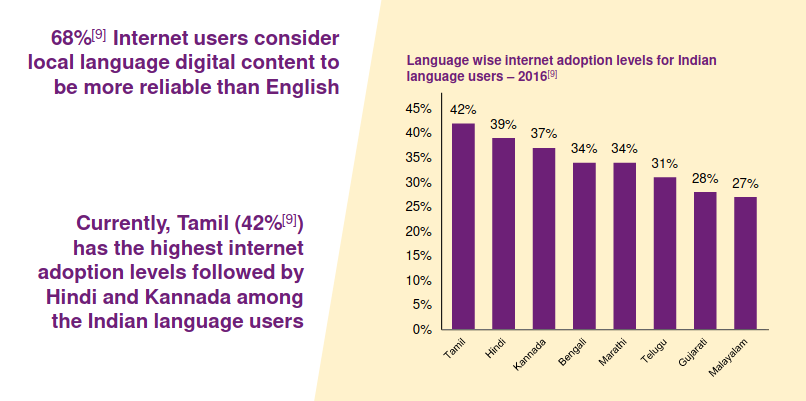
\includegraphics[width=\textwidth]{localrel}

Access to the internet in a native language brings with it not only the expanse
of content provided to the user in said native tongue, but also access to the
vast and open nature of the internet in itself. Collaborative encyclopaedias,
open access to the latest state of the art in technological advancements, the
wide world of open source. By enabling native language content on the internet,
it enriches the lives of both those inducted and those inducting.

A key feature that should not be forgotten here is the incredible growth the
vast multitudes of multilingual data will provide to researchers working in
Information Retrieval and Natural Language Processing, enabling them to better
overcome the problem of data sparsity. And the data will, for a while anyway,
definitely never be enough -- as seen in recent times, from 340 million
parameters in BERT \cite{devlin_bert_2019}, to the 1.5 billion parameters in
GPT-2 \cite{radford_language_2019}, all the way up to 150 billion in GPT-3
\cite{brown_language_2020}, at which there is still no end in sight,
Transformers get better the more data they get.

What that means is that due to the increased amount of language data and more
users of said language, the tools to improve accessibility from outside to
enable the users to explore far more of the internet than was previously
possible, engaging other users to join and generate more content which in turn
improves the systems further and further and on and on and so on.

But what does that \textit{actually} mean? In case you have read the fantastic
Hitchhikers Guide to the Galaxy, this means we functionality can get to the
point of having a babel fish. From the lowered, demeaned status of stragglers on
the internet highways suddenly everybody is upgraded to first class status, able
to access and read and understand anything written in any language, including
the highly abundant English side of the internet. Not to exploit the Library of
Alexandria metaphor \textit{too} much, but -- I mean -- the modern Library of
Alexandria, at one's fingertips.

(It should go without saying that the vision described here is as far into the
future as Artificial General Intelligence (AGI), and it is incredibly unlikely
that the state of AI as it is today will be able to reach those staggering
heights. Yet, are we not already there to an extent? Consider how often we use
Google translate's "Translate this page" to read an Arabic news report about our
favourite football team. If such small steps are a reality now, it is not
impossible to imagine a future -- not a perfect one, perhaps, but one that
exists \textit{pretty darn well} for what it is.)

\subsubsection{Education}

And then we come to Education. A contentious topic, one that many have wrapped
their heads around, many with far worthier heads than yours or mine. And yet,
the results remain untold, every new batch of students one untested experiment
after the other. Will discipline hold them in? Perhaps... more medieval methods? 
It appears
not, as it is now the twenty first century, and yet newer batches have been
ushered in for experimentation after those of the last few decades never managed
to catch on to a winning formula.

One of these debates is about the \textit{language of education}. It has always
been the case. Wherever be a conflict of language, there will be the argument of
what should be taught at school? The answer may not be as simple as we may make
it seem due to the plays and tricks of politics, but skipping over such for the
day we move into the seemingly simple question of, what's better for the child?

You might recall the earlier "Major Insight" where we claimed "undeniably" that
one's native tongue was best suited to educate themselves to the best of their
intellectual capacity. That was not entirely conjured out of thin air and
misdirection. Research has suggested \cite{hudelson_role_1987} that one's Native
tongue when used when educating at the primary level benefits children's
development in classrooms. Others have also spoken of the benefits of fluency in
bilingual education, rather than eradicating the native tongue for English
\cite{hakuta_compendium_1986} \cite{cummins_bilingualism_1981}. 

Students from the UG2k17 batch may in fact remember something else related to
the issue - a series of 2 Theory of Knowledge lectures during induction by
Professor Harjinder Singh (Laltu). In this series of lectures, the focus was on
how humans -- here, specifically Indians -- would benefit from being taught in
their "mother tongue" for the first few years of primary education
\cite{noauthor_knowledge_2020}. This may also seem familiar to those who have
not attended this lecture series - the National Educational Policy (NEP) 2020
announced a very similar plan, of requiring education in the mother/regional
tongue through elementary level.

So how does this tie into the need for content in native tongues on the
internet? Education is not limited to the classroom -- the internet is rife with
avenues for learning. Particularly in the form of both videos and text,
native-language information is more digestible to a populace more familiar with
their own tongue. Consider the absolute carnage of Hindi video tutorials on
youtube, and their popularity that surpasses even some of the biggest "Youtube
celebrities" with their international appeal with English. The content is still
language-locked -- in that the content cannot be consumed outside of the
boundaries of the language itself, but to those that could not access other
tutorials and lectures earlier, now there is a way to learn. 

Now let us take this goldmine of content yet again with the lens of IR and NLP
-- with more data, comes better models. With better models, come better systems.
With better systems, inter and intra language tasks become more accurate, more
reliable, more generically usable. A Bengali kid can now tap into this system
and watch English MOOC content, without knowing a word of the language. Okay,
some of it is needed, but they're borrowed words anyway so it does not
particularly matter as much. The point is that the information of all of the
internet, in its previously untapped potential, is now available to anyone who
is able to access content in their own native tongue.

\subsubsection{Culture}

One oft-forgotten aspect of the social fabric is culture -- here, more
specifically, how language content available on the internet will enable
cultural conversion and exploration in ways previously imaginable. To quote
\cite{geser_digicult_2002}, "The conversion of all sorts of cultural contents 
into bits and bytes opens up a completely new dimension of reaching traditional 
and new audiences by providing access to cultural heritage resources in ways 
unimaginable a decade ago".  The digital age allows access to tools and methods
previously never thought of, to not port a language and its associated culture
to the interwebs would be quite the disaster.

\subsection{Political}

There are political arguments to be made as well.

English is often considered by many to be the language of the "elite" -- the
landed, casted upper classes, protégés of the Imperial system of education in
all but name. It's a common slur of sorts, cast at those who speak English,
hints of Lutyen's in the attacks. 

Even among those not going to such extremes -- it is, after all, the twenty 
first century -- it is a common refrain that the politics of the rich is
inaccessible, precisely because it is only available in one language -- English
-- a language inaccessible to those not in the upper echelons of a casted
society, and even when available, restricted through accent and fluency to
create an artificial class divide. Such is the claim, of English as the "elite
persons language".

To avoid that, information needs to be in native tongues too. Be it the
Communist Manifesto or Atlas Unshrugged, the mass appeal comes from its far more
accessible to many translations.

\subsection{Economic}

It just so happens that the same people who use the internet to learn, talk, and
so on and so forth will also happen to use the very same internet for online
shopping, and visiting websites that sell things, even if not physically for
money at the very spot.

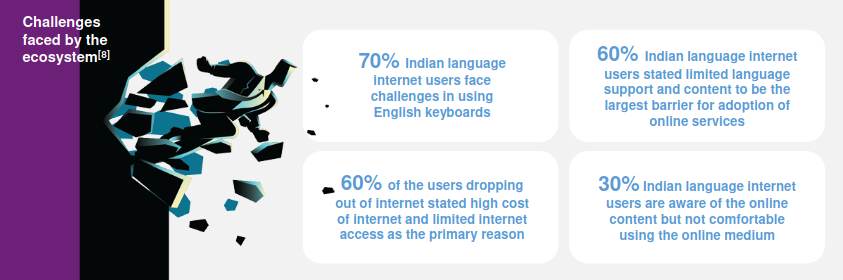
\includegraphics[width=\textwidth]{indlang}

It also happens thus, by adding a language-specific version of the website, user
checkout and interaction goes through the roof. Which is again, not too
surprising -- most areas have some local language along with a more "formal"
one, often English, where the formal one is more a rarity and the local, the
language of the masses. E-commerce would be expected to be more in the local
versions of these websites, sometimes in large enough regions that substantial
profits can be made off of the addition of the language-native search and
operation options.

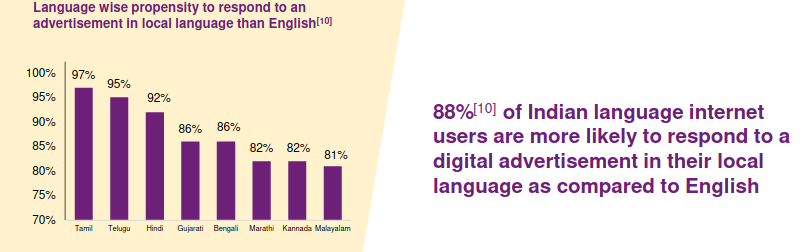
\includegraphics[width=\textwidth]{indad}

\section{Conclusions}

The employment of local or native languages across the internet is still as of
date, like most of the internet, voluntary, albeit sometimes funded by State
governments in order to promote said language. That said, it is a pursuit worth
pursuing, not only for the benefit of Deep Learning systems requiring more data,
but also for humans.

% include your own bib file like this:
% \bibliographystyle{coling}
% \bibliography{coling2020}

\bibliographystyle{coling}
\bibliography{ireterm}

%\begin{thebibliography}{}

%\bibitem[\protect\citename{Aho and Ullman}1972]{Aho:72}
%Alfred~V. Aho and Jeffrey~D. Ullman.
%\newblock 1972.
%\newblock {\em The Theory of Parsing, Translation and Compiling}, volume~1.
%\newblock Prentice-{Hall}, Englewood Cliffs, NJ.

%\bibitem[\protect\citename{{American Psychological Association}}1983]{APA:83}
%{American Psychological Association}.
%\newblock 1983.
%\newblock {\em Publications Manual}.
%\newblock American Psychological Association, Washington, DC.

%\bibitem[\protect\citename{{Association for Computing Machinery}}1983]{ACM:83}
%{Association for Computing Machinery}.
%\newblock 1983.
%\newblock {\em Computing Reviews}, 24(11):503--512.

%\bibitem[\protect\citename{Chandra \bgroup et al.\egroup }1981]{Chandra:81}
%Ashok~K. Chandra, Dexter~C. Kozen, and Larry~J. Stockmeyer.
%\newblock 1981.
%\newblock Alternation.
%\newblock {\em Journal of the Association for Computing Machinery},
%  28(1):114--133.

%\bibitem[\protect\citename{Gusfield}1997]{Gusfield:97}
%Dan Gusfield.
%\newblock 1997.
%\newblock {\em Algorithms on Strings, Trees and Sequences}.
%\newblock Cambridge University Press, Cambridge, UK.

%\bibitem[\protect\citename{Rasooli and Tetreault}2015]{rasooli-tetrault-2015}
%Mohammad~Sadegh Rasooli and Joel~R. Tetreault. 2015.
%\newblock {Yara parser: {A} fast and accurate dependency parser}.
%\newblock \emph{Computing Research Repository}, arXiv:1503.06733.
%\newblock Version 2.

%\bibitem[\protect\citename{Borschinger and Johnson}2011]{borsch2011}
%Benjamin Borschinger and Mark Johnson. 2011.
%\newblock A particle filter algorithm for {B}ayesian wordsegmentation.
%\newblock In \emph{Proceedings of the Australasian Language Technology Association %Workshop 2011}, pages 10--18, Canberra, Australia.

%\end{thebibliography}

\end{document}
